%% Based on a TeXnicCenter-Template by Tino Weinkauf.
%%%%%%%%%%%%%%%%%%%%%%%%%%%%%%%%%%%%%%%%%%%%%%%%%%%%%%%%%%%%%

%%%%%%%%%%%%%%%%%%%%%%%%%%%%%%%%%%%%%%%%%%%%%%%%%%%%%%%%%%%%%
%% HEADER
%%%%%%%%%%%%%%%%%%%%%%%%%%%%%%%%%%%%%%%%%%%%%%%%%%%%%%%%%%%%%
\documentclass[a4paper,oneside,12pt]{report}
% Alternative Options:
%	Paper Size: a4paper / a5paper / b5paper / letterpaper / legalpaper / executivepaper
% Duplex: oneside / twoside
% Base Font Size: 10pt / 11pt / 12pt


%% Language %%%%%%%%%%%%%%%%%%%%%%%%%%%%%%%%%%%%%%%%%%%%%%%%%
\usepackage[USenglish]{babel} %francais, polish, spanish, ...
\usepackage[T1]{fontenc}
\usepackage[ansinew]{inputenc}

\usepackage{lmodern} %Type1-font for non-english texts and characters


%% Packages for Graphics & Figures %%%%%%%%%%%%%%%%%%%%%%%%%%
\usepackage{graphicx} %%For loading graphic files
%\usepackage{subfig} %%Subfigures inside a figure
%\usepackage{pst-all} %%PSTricks - not useable with pdfLaTeX

%% Please note:
%% Images can be included using \includegraphics{Dateiname}
%% resp. using the dialog in the Insert menu.
%% 
%% The mode "LaTeX => PDF" allows the following formats:
%%   .jpg  .png  .pdf  .mps
%% 
%% The modes "LaTeX => DVI", "LaTeX => PS" und "LaTeX => PS => PDF"
%% allow the following formats:
%%   .eps  .ps  .bmp  .pict  .pntg


%% Math Packages %%%%%%%%%%%%%%%%%%%%%%%%%%%%%%%%%%%%%%%%%%%%
\usepackage{amsmath}
\usepackage{amsthm}
\usepackage{amsfonts}


%% Line Spacing %%%%%%%%%%%%%%%%%%%%%%%%%%%%%%%%%%%%%%%%%%%%%
%\usepackage{setspace}
%\singlespacing        %% 1-spacing (default)
%\onehalfspacing       %% 1,5-spacing
%\doublespacing        %% 2-spacing


%% Other Packages %%%%%%%%%%%%%%%%%%%%%%%%%%%%%%%%%%%%%%%%%%%
%\usepackage{a4wide} %%Smaller margins = more text per page.
%\usepackage{fancyhdr} %%Fancy headings
%\usepackage{longtable} %%For tables, that exceed one page
\usepackage{enumerate}

%%%%%%%%%%%%%%%%%%%%%%%%%%%%%%%%%%%%%%%%%%%%%%%%%%%%%%%%%%%%%
%% Remarks
%%%%%%%%%%%%%%%%%%%%%%%%%%%%%%%%%%%%%%%%%%%%%%%%%%%%%%%%%%%%%
%
% TODO:
% 1. Edit the used packages and their options (see above).
% 2. If you want, add a BibTeX-File to the project
%    (e.g., 'literature.bib').
% 3. Happy TeXing!
%
%%%%%%%%%%%%%%%%%%%%%%%%%%%%%%%%%%%%%%%%%%%%%%%%%%%%%%%%%%%%%

%%%%%%%%%%%%%%%%%%%%%%%%%%%%%%%%%%%%%%%%%%%%%%%%%%%%%%%%%%%%%
%% Options / Modifications
%%%%%%%%%%%%%%%%%%%%%%%%%%%%%%%%%%%%%%%%%%%%%%%%%%%%%%%%%%%%%

%\input{options} %You need a file 'options.tex' for this
%% ==> TeXnicCenter supplies some possible option files
%% ==> with its templates (File | New from Template...).



%%%%%%%%%%%%%%%%%%%%%%%%%%%%%%%%%%%%%%%%%%%%%%%%%%%%%%%%%%%%%
%% DOCUMENT
%%%%%%%%%%%%%%%%%%%%%%%%%%%%%%%%%%%%%%%%%%%%%%%%%%%%%%%%%%%%%
\begin{document}

\pagestyle{empty} %No headings for the first pages.


%% Title Page %%%%%%%%%%%%%%%%%%%%%%%%%%%%%%%%%%%%%%%%%%%%%%%
%% ==> Write your text here or include other files.

%% The simple version:
\title{ECE 5566 Assignment IV}
\author{Ramakrishnan Kalyanaraman\\
VT ID: 905782081\\
PID: rk126}
%\date{} %%If commented, the current date is used.
\maketitle

\begin{center}
	\section*{ECE/CS 5566 HW 4}
\end{center}

\begin{figure}[h!]
  \centering
    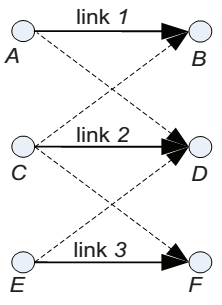
\includegraphics[width=0.3\textwidth]{fig_1}
	\caption{A 6-node network with 3 active links in time slot t}
\end{figure}

Consider a 6-node network in Fig. 1, where each node is equipped with 4 antennas. Suppose in time slot t, there are 3 active links as shown in the figure, where a solid line represents a directed link and a dashed arrow represents interference. Denote $\phi(t)=(z_1 (t),z_2 (t),z_3 (t))$ as the number of data streams on the three active links.	\\*

\textbf{Problem 1}	\\*

Suppose that we want to determine the feasibility of $\phi(t)=(1,2,1)$ using the matrix-based model.

\begin{enumerate} [(i)]

\item	(+2 points) How many transmit and receive vectors are needed for $\phi(t)$?

For each data stream we have one transmit vector and one receive vector. Hence we have,
1 transmit vector for transmit node A and 1 receive vector for receive node B,
2 transmit vector for transmit node C and 2 receive vector for receive node D,
1 transmit vector for transmit node E and 1 receive vector for receive node F.
Hence for $\phi(t)$, we have 4 transmit vectors and 4 receive vectors.

\item	(+2 points) What is the total number of variables that are involved in the transmit and the receive vectors?

The total number of variables involved in the transmit and the receive vectors is given by,

$$2 \times (Z_1(t) + Z_2(t) + Z_3(t)) \times A$$

We are multiplying with a 2 because we are considering variables involved at both transmit and receive nodes respectively.

$2 \times (1 + 2 + 1) \times 4 = 32$ variables

\item	(+4 points) How many bilinear equations do we need to solve to determine the feasibility of $\phi(t)=(1,2,1)$? Show details.

We need to solve $$1^2 + 2^2 + 1^2 + 1 \times 2 + 2 \times 1 + 1 \times 2 + 2 \times 1 = 14$$ equations

Here, u represents transmit vector, V represents receive vector and $H_l$ represents the link matrix of link l. Subscript represents the link number and the superscript represents the data stream number.

Spatial Multiplexing in link 1:

Since, $Z_1(t) = 1$, we have,

$$(u^1_1)^T H_1 V^1_1 = 1$$

Spatial Multiplexing in link 2:

Since, $Z_2(t) = 2$, we have,

$$(u^1_2)^T H_2 V^1_2 = 1$$

$$(u^2_2)^T H_2 V^2_2 = 1$$

$$(u^2_2)^T H_2 V^1_2 = 0$$

$$(u^1_2)^T H_2 V^2_2 = 0$$

Spatial Multiplexing in link 3:

Since, $Z_3(t) = 1$, we have,

$$(u^1_3)^T H_1 V^1_3 = 1$$

Interference cancellation in link from A to D, we call it "4"

Both link 1 and link 2 involving data streams $Z_1(t) = 1$ and $Z_2(t) = 2$

$$(u^1_1)^T H_4 V^1_2 = 0$$

$$(u^1_1)^T H_4 V^2_2 = 0$$

Interference cancellation in link from C to B, we call it "5"

Both link 1 and link 2 involving data streams $Z_1(t) = 1$ and $Z_2(t) = 2$

$$(u^1_2)^T H_5 V^1_1 = 0$$

$$(u^2_2)^T H_5 V^1_1 = 0$$

Interference cancellation in link from C to F, we call it "6"

Both link 2 and link 3 involving data streams $Z_2(t) = 2$ and $Z_3(t) = 1$

$$(u^1_2)^T H_6 V^1_3 = 0$$

$$(u^2_2)^T H_6 V^1_3 = 0$$

Interference cancellation in link from E to D, we call it "7"

Both link 2 and link 3 involving data streams $Z_2(t) = 2$ and $Z_3(t) = 1$

$$(u^1_3)^T H_7 V^1_2 = 0$$

$$(u^1_3)^T H_7 V^2_2 = 0$$

\end{enumerate}

\textbf{Problem 2}	\\*

\begin{enumerate} [(i)]

\item (+8 points) Suppose that we want to determine the feasibility of $\phi(t)=(1,2,1)$ using the node-ordering based DoF model. For a given node ordering $\pi=[C B D A E F]$, is $\phi(t)$ feasible? Show all details.

We have $A = 4$, which is the number of antennas present at each node. This number also represents the total number of resources present at each node.

Each node has to consume resources for two purposes,
\begin{enumerate}
	\item Spatial Multiplexing (SM)
	\item Interference Cancellation (IC)
\end{enumerate}

This total number of resources spent on SM and IC should not exceed the actual number of resources present at each node, which is 4 (number of antennas) for each node. Number of data streams for each desired communication link given by $\phi(t)$ are as follows,

$Z_1(t) = 1, Z_2(t) = 2, Z_3(t) = 1$

From the order given in $\pi$, we start,

For Spatial Multiplexing at each nodes, the number of resources spent by each node equals to the number of data streams associated with that node's actual communication link. Hence, the number of DoFs consumed for spatial multiplexing is given in the table below.

For Interference Cancellation at each nodes,

C: 1st Transmit Node

No receive node(s) present before the transmit node C which is the first one in the given order. Hence, we don't have to consume any DoF for Interference cancellation.

B: 2nd Receive Node

B has a transmit node C which is in the interference region of B before itself in the given order. Hence, it consumes 2 DoF to cancel interference from node C. Since, $Z_2(t) = 2$

D: 3rd Receive Node

Transmit node C comes before the receive node D in the given order. But it has an "desired" communication link with C and NOT an interference. Hence it doesn't consume any DoF for Interference Cancellation.

A: 4th Transmit Node

Receive Node B and D falls before this node in the given order. B is an "desired" receive node and NOT an interference. Whereas, receive node D is in the interference range of transmit node A. Hence, A consumes 2 DoF resource to cancel interference caused to node D. It is 2 because $Z_2(t) = 2$ is the number of data streams desired by the Receive node D.

E: 5th Transmit Node

Receive Node B and D falls before this node in the ordered list. B is not in the interference range of E. Whereas, receive node D is in the interference range of E. Hence, it will use 2 DoF resources to cancel that interference caused to node D. It is 2 because $Z_2(t) = 2$ is the number of data streams desired by the Receive node D.

F: 6th Receive Node

Transmit node A, C and E respectively are before receive node F.
But, A is out of the interference range of F,
E is the desired transmit node for receive node F,
Node F will use 2 DoF ($Z_2(t) = 2$) resources for interference cancellation from node C.

Therefore,

\begin{center}
  \begin{tabular}{ l | l | l | l | l | l | l }
    \hline
		0			& C & B & D & A & E & F \\ \hline
    SM 		& 2 & 1 & 2 & 1 & 1 & 1 \\ \hline
    IC 		& 0 & 2 & 0 & 2 & 2 & 2 \\ \hline
		Total & 2 & 3 & 2 & 3 & 3 & 3	\\ \hline
  \end{tabular}
\end{center}

Since, the total resources consumed by any of the node doesn't exceed the value of A (which is 4), the given order $\pi=[C B D A E F]$, $\phi(t) = (1, 2, 1)$ is \textbf{feasible}.

\item (+8 points) Suppose that we want to determine the feasibility of $\phi(t)=(1,2,1)$ using the node-ordering based DoF model. For a given node ordering $\pi=[C B D A E F]$, is $\phi(t)$ feasible? Show all details.

We have $A = 4$, which is the number of antennas present at each node. This number also represents the total number of resources present at each node.

Each node has to consume resources for two purposes,
\begin{enumerate}
	\item Spatial Multiplexing (SM)
	\item Interference Cancellation (IC)
\end{enumerate}

This total number of resources spent on SM and IC should not exceed the actual number of resources present at each node, which is 4 (number of antennas) for each node. Number of data streams for each desired communication link given by $\phi(t)$ are as follows,

$Z_1(t) = 1, Z_2(t) = 3, Z_3(t) = 2$

From the order given in $\pi$, we start,

For Spatial Multiplexing at each nodes, the number of resources spent by each node equals to the number of data streams associated with that node's actual communication link. Hence, the number of DoFs consumed for spatial multiplexing is given in the table below.

For Interference Cancellation at each nodes,

C: 1st Transmit Node

No receive node(s) present before the transmit node C which is the first one in the given order. Hence, we don't have to consume any DoF for Interference cancellation.

B: 2nd Receive Node

B has a transmit node C which is in the interference region of B before itself in the given order. Hence, it consumes 3 DoF to cancel interference from transmit node C. Since, transmit node C's desired communication link's number of data stream is $Z_2(t) = 3$

D: 3rd Receive Node

Transmit node C comes before the receive node D in the given order. But it has an "desired" communication link with C and NOT an interference. Hence it doesn't consume any DoF for Interference Cancellation.

A: 4th Transmit Node

Receive Node B and D falls before this node in the given order. B is an "desired" receive node and NOT an interference. Whereas, receive node D is in the interference range of transmit node A. Hence, A consumes 3 DoF resource to cancel interference caused to node D. It is 3 because $Z_2(t) = 3$ in the desired link of the Receive node D.

E: 5th Transmit Node

Receive Node B and D falls before this node in the ordered list. B is not in the interference range of E. Whereas, receive node D is in the interference range of E. Hence, it will use 3 DoF resources to cancel that interference caused to node D. It is 3 because $Z_2(t) = 3$ in the desired link of the Receive node D.

F: 6th Receive Node

Transmit node A, C and E respectively are before receive node F.
But, A is out of the interference range of F,
E is the desired transmit node for receive node F,
Node F will use 3 DoF ($Z_2(t) = 3$) resources for interference cancellation from node C.

Therefore,

\begin{center}
  \begin{tabular}{ l | l | l | l | l | l | l }
    \hline
		0			& C & B & D & A & E & F \\ \hline
    SM 		& 3 & 1 & 3 & 1 & 2 & 2 \\ \hline
    IC 		& 0 & 3 & 0 & 3 & 3 & 3 \\ \hline
		Total & 3 & 4 & 3 & 4 & 5 & 5	\\ \hline
  \end{tabular}
\end{center}

Since, the total resources consumed by any of the node exceeds the value of A (which is 4) specifically for node E and F, the given order $\pi=[C B D A E F]$, $\phi(t) = (1, 3, 2)$ is \textbf{unfeasible}.

\end{enumerate}

\end{document}

